%% SW design: PSoC Domain

\begin{figure}[htbp] \centering
{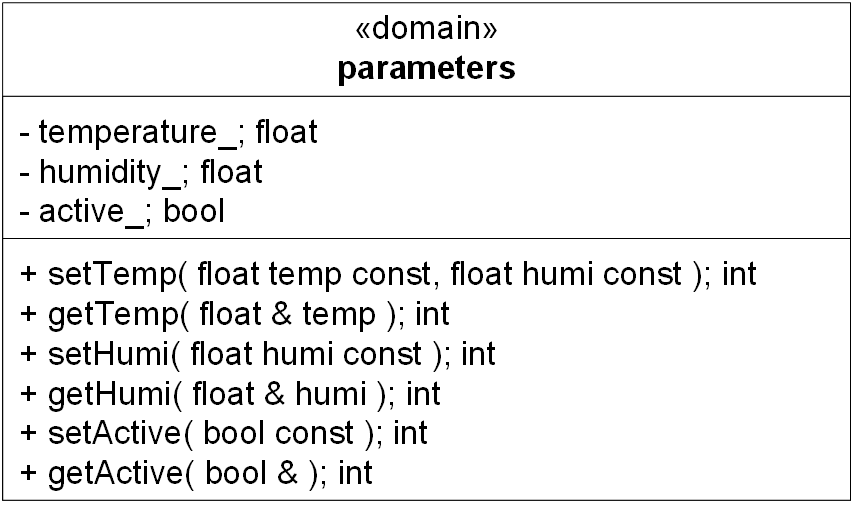
\includegraphics[scale=1.3]{filer/design/Klassediagrammer/sw_psoc_parameters}}
\caption{Klasse parameters}
\label{fig:sw_psoc_class_parameters}
\end{figure} 

{\centering
\textbf{parameters}\par
}
\textbf{Ansvar:} Gemme information om grænseværdier mv. til det autonome vandingssystem. \

\textbf{Attributter:}
\begin{itemize}
	\item \verb+float temperature_+ Øvre temperaturgrænse
	\item \verb+float humidity_+ Nedre fugtighedsgrænse
	\item \verb+unsigned char active_+ Flag for om vanding er aktiv eller ikke
\end{itemize}

\verb+void init( parameters * const this ) +\\
\textbf{Parametre:} Pointer til aktuelt objekt. \\
\textbf{Returværdi:} Ingen. \\
\textbf{Beskrivelse:} Initialiserer medlemsattributterne: \verb+active_+: 1, \verb+humidity_+: 10 og \verb+temperature_+: 30. \\

\verb+int setTemp( parameters * const this, const float temp ) +\\
\textbf{Parametre:} Temperatur. \\
\textbf{Returværdi:} 0 ved succes ellers negativ i overenstemmelse med fejl-listen. \\
\textbf{Beskrivelse:} Gemmer modtagne data i medlem \verb+temperature_+. \\

\verb+int getTemp( parameters * const this, float * temp )+ \\
\textbf{Parametre:} Pointer til at gemme data i. \\
\textbf{Returværdi:} 0 ved succes ellers negativ i overenstemmelse med fejl-listen. \\
\textbf{Beskrivelse:} Returnerer medlem \verb+temperature_+ i modtagne pointer. \\

\verb+int setHumi( parameters * const this, const float humi )+ \\
\textbf{Parametre:} Humidity. \\
\textbf{Returværdi:} 0 ved succes ellers negativ i overenstemmelse med fejl-listen. \\
\textbf{Beskrivelse:} Gemmer modtagne data i medlem \verb+humidity_+. \\

\verb+int getHumi( parameters * const this, float * humi )+ \\
\textbf{Parametre:} Pointer til at gemme data i. \\
\textbf{Returværdi:} 0 ved succes ellers negativ i overenstemmelse med fejl-listen. \\
\textbf{Beskrivelse:} Returnerer medlem \verb+humidity_+ i modtagne pointer. \\

\verb+int setActive( parameters * const this, const unsigned char )+ \\
\textbf{Parametre:} 1 = aktiv, 0 = inaktiv. \\
\textbf{Returværdi:} 0 ved succes ellers negativ i overenstemmelse med fejl-listen. \\
\textbf{Beskrivelse:} Gemmer modtagne data i medlem \verb+active_+. \\

\verb+int getActive( parameters * const this, unsigned char * )+ \\
\textbf{Parametre:} Pointer til at gemme data i. \\
\textbf{Returværdi:} 0 ved succes ellers negativ i overenstemmelse med fejl-listen. \\
\textbf{Beskrivelse:} Returnerer medlem \verb+active_+ i modtagne pointer. \\


\begin{figure}[htbp] \centering
{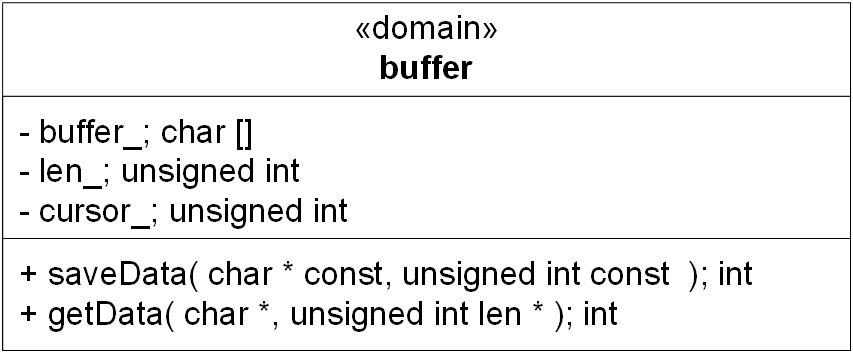
\includegraphics[scale=1.3]{filer/design/Klassediagrammer/sw_psoc_buffer}}
\caption{Klasse buffer}
\label{fig:sw_psoc_class_buffer}
\end{figure} 

{\centering
\textbf{buffer}\par
}
\textbf{Ansvar:} Holde data fra sensorerne indtil de udlæses af Master. Gemmer også fejlbeskeder fra systemet. \

\textbf{Attributter:}
\begin{itemize}
	\item \verb+char buffer_[]+ Array til at holde 1 datalæsning og 10 fejl.
	\item \verb+unsigned int len_+ Længden på arrayet
	\item \verb+unsigned int cursor_+ Index på næste frie plads i array
	\item \verb+unsigned int dataIndex_+ Index på placering af data i array, hvis der tidligere har været gemt data
	\item \verb+unsigned char dataWritten_+ Flag til at indikerer tidligere skrevet data
\end{itemize}

\verb+void buffer( buffer * )+ \\
\textbf{Parametre:} Pointer til aktuelt objekt. \\
\textbf{Returværdi:} Ingen. \\
\textbf{Beskrivelse:} r \verb+char+ array \verb+buffer_+ med plads til én datamåling og 10 fejl, iht. dataprotokol, \ref{header:dataprotokol}, til 0. Initialiserer også medlemmer til 0 på nær \verb+len_+ som initialiseres til arrayets længde \verb+BUFFER_LENGTH+.\\

\verb+int saveData( buffer * const, const char * buf, const unsigned int len )+ \\
\textbf{Parametre:} Pointer til aktuelt objekt og pointer til buffer med len data. \\
\textbf{Returværdi:} 0 ved succes ellers negativ i overenstemmelse med fejl-listen. \\
\textbf{Beskrivelse:} Gemmer modtaget data i array, hvis der er plads til det. Hvis det er en data-logning, kontrolleres der om der ligger en ældre måling i bufferen, som i så fald overskrives. Markøren flyttes iht. hvor meget der skrives ind. \\

\verb+int getData( buffer * const, char ** buf, unsigned int * len )+ \\
\textbf{Parametre:} Pointer til aktuelt objekt og pointer til char array til data. \\
\textbf{Returværdi:} 0 ved succes ellers negativ i overenstemmelse med fejl-listen. \\
\textbf{Beskrivelse:} Returnerer pointeren til array i \verb+buf+ og \verb+cursor_+ i \verb+len+. Nulstiller derefter \verb+cursor_+ og \verb+dataWritten_+.\\